

\chapter{Testing methodology}
\label{chap:method}

The initial RepNet framework, as described by \textit{Rens et al.} \cite{rensetal}, was developed as a novel extension to the standard POMDP framework, but was subsequently left unimplemented. \RefChap{chap:mdp} covered the simplification process of the RepNet framework to a fully observable setting, in an effort to reduce its intractability. The chapter furthermore discussed an alternative to exact planning such as \textit{value iteration}, called \textit{approximate online} planning, in the context of the simplified RepNet framework. More concretely, a look-ahead search algorithm can be used to approximate the real value function given the current \textit{epistemic state} (\RefSec{sec:onlineplan}). The goal of the present chapter is to present the experimental setup devised to test the framework's properties. \RefSec{sec:testbed} introduces the \textit{scenarios} used to showcase the working principles of the RepNet framework. \RefSec{sec:expset} then details the actual experimental setup. Finally, \RefSec{sec:params} discusses the settings for the parameters that are common across all experiments, while \RefSec{sec:specif} covers the experiment-dependent parameters.

\section{Test bed}
\label{sec:testbed}
This section outlines the \textit{scenarios} that make up the entirety of the experimental setup. Each scenario was designed to showcase specific elements of the RepNet framework. Two types of scenarios are considered in this thesis: \textit{Trading} and \textit{Air-taxi} scenarios. All scenarios are used for different purposes and highlight different aspects of the framework.

\subsection{Trading scenarios}
A \textit{trade transaction} is the activity by which a first party, called the \textit{buyer}, wishes to buy a good from a second party, called the \textit{seller}. A trade transaction materializes when the buyer is willing to buy, and the seller is willing to sell. The trading scenarios used in this thesis involve two to three agents and are designed to showcase the interaction between RepNet and non-RepNet agents.
The first trading scenario, described in \RefEx{ex:trade2ag}, involves two agents and is schematized in \RefFig{fig:ex111}. As the scenario involves only a small number of states, its corresponding transition model is furthermore depicted in \RefFig{fig:ex1}.
\begin{example}[Trade transaction between two agents]
\label{ex:trade2ag}
Let $A$ and $B$ be two agents. Agent $A$ plays the role of the buyer, agent $B$ the role of the seller. Agent $A$ can engage in a trade with agent $B$, and $B$ can accept or refuse the trade offer. Furthermore, agent $A$ can, prior to making a trade offer, do a good deed in an effort to improve its image in the eyes of agent $B$. 
\end{example}
\begin{figure}[h]
    \centering
    \includegraphics[width=0.35\textwidth]{images/MasterThesisVTOL2agDrawOther.pdf}
    \caption{Trading scenario with two autonomous agents. Agent $A$ can make trade offers, which agent $B$ can accept or refuse.}
    \label{fig:ex111}
\end{figure}
\begin{figure}[h]
    \centering
    \includegraphics[width=0.75\textwidth]{images/MasterThesisTrade2AgDraw (1).pdf}
    \caption{Transition model of the Trading scenario between agents $A$ and $B$. Node 0 is the starting state, node 1 is the state following agent $A$'s good deed, nodes 2 and 3 are states in which agent $A$ has made an offer and is waiting for $B$'s response, and nodes 4 is the \textit{accept} state.}
    \label{fig:ex1}
\end{figure}



The second trading scenario, described in \RefEx{ex:trade3ag}, involves three agents. The scenario is schematized in \RefFig{fig:ex2}.

\begin{example}[Trading between three agents]
\label{ex:trade3ag}
Let $A$, $B$, and $C$ be three agents. Each agent simultaneously plays the role of buyer and seller, and can thus engage in a trade with any other agent. Each agent can accept or refuse any trade offer made by any remaining agent.
\end{example}
\begin{figure}[h]
  \begin{center}
    \includegraphics[width=0.31\textwidth]{images/MasterThesistrade3agDraw (3).pdf}
  \end{center}
  \caption{Trading scenario with 3 autonomous agents, each agent can \texttt{trade} with any remaining agent, \texttt{accept}, and \texttt{refuse} trade offers}\label{fig:ex2}
\end{figure}

\subsection{Air-taxi (eVTOL) scenarios}
Electric Vertical Take-off and Landing (eVTOL) aircraft are electric powered aircraft that can can take-off and land vertically, meaning they do not require a runway, and can hover at a given altitude \cite{vtol,vtol56}. Recently, several big companies, including Boeing and NASA, Uber and Lilium GmbH have invested large amounts of money into the development of eVTOL aircraft designed to provide taxi services in and out of cities \cite{vtol2, vtol3}.
These pilotless aircraft make up a network of agents that require air traffic management. Simplified air-taxi scenarios are used in the experimental setup, and are described hereafter.
The first and simplest air-taxi scenario is given in \RefEx{ex:air1} and involves two agents. The scenario is schematized in \RefFig{fig:ex3}.
\begin{example}[Air-taxi battery level management]
\label{ex:air1}
The airspace considered in this example is made up of 1 vertiport, i.e., airport for eVTOL aircraft, as well as a common flying space. The network is made up of 2 eVTOL aircraft, and each aircraft has 3 battery levels (high, medium, low). Upon landing at a vertiport, the battery of an aircraft is fully recharged. A central unit called an oracle, receives the position and battery level of each aircraft at every time-step, and immediately distributes the information to the entire network, thereby bringing the problem to a fully observable setting. At any point in time, only one aircraft may use the vertiport. Each agent's goal is to not run out of battery in the air. The selfish incentive would, therefore, appear to be to stay at the vertiport. This would, however, prevent the other agent from using that same platform, possibly when they most need to. The combined constraint, therefore, lies in the fact that no aircraft may crash at any point in time.
\end{example}

\begin{figure}[h]
  \begin{center}
    \includegraphics[width=0.5\textwidth]{images/MasterThesisVTOL2agDraw (2).pdf}
  \end{center}
  \caption{Air-taxi scenario with 2 autonomous agents}\label{fig:ex3}
\end{figure}



The second air-taxi scenario, detailed in \RefEx{ex:air2}, involves 4 agents and figures as the most complex example. A scheme of the scenario is given in \RefFig{fig:ex4}.


\begin{example}[Air-taxi travel]
\label{ex:air2}
The airspace considered in this example is designed as a grid that includes 4 vertiports. The network is made up of 4 eVTOL aircraft/agents, each aircraft assumed to have infinite battery. The goal of each agent is to travel to their assigned vertiport along a fixed itinerary, without crashing into any other aircraft. At the start of a run, these agents are randomly placed on the grid somewhere along their axis of travel. Each agent is fully aware of every agent's position on the grid, making the problem fully observable. The selfish goal resides in the fact that each agent wishes to reach their vertiport as quickly as possible. In doing so, the risk of two agents crashing into each other is increased substantially. Agents are, therefore, required to be cooperative, in spite of their selfish intentions \cite{2590}.

\end{example}


\begin{figure}[h]
  \begin{center}
    \includegraphics[width=0.48\textwidth]{images/MasterThesisVTOL4Draw (2).pdf}
  \end{center}
  \caption{Air-taxi scenario with 4 autonomous agents}\label{fig:ex4}
\end{figure}


\section{Experimental setup}
\label{sec:expset}
The scenarios described in \RefSec{sec:testbed} are used in a series of experiments designed to test different aspects of the RepNet framework. Concretely, the experimental setup is divided into three parts, which are discussed in the present section. \RefSec{sub:repfeat} deals with tests conducted to test the main properties of the RepNet framework. In \RefSec{sub:adaptrep}, the ability of RepNet agents to quickly adapt to changes in other agents' behavior is discussed. Finally, \RefSec{sub:largescale} extends the experimental setup to include more than two agents.

\subsection{The RepNet framework features}
\label{sub:repfeat}
The first part of the experimental evaluation concerns itself with testing the properties that distinguish RepNet-MDPs from other MDP-derived frameworks, and are thus conducted without the presence of a baseline framework. As a reminder, the properties of the RepNet framework include the notions of \textit{action distribution}, \textit{image}, \textit{reputation}, and \textit{directed actions}. The first series of experiments addresses the first three features, while the second one showcases the benefits and drawbacks of using directed actions. Both series of experiments take part in the environment described in \RefEx{ex:trade2ag}.

\subsubsection{Testing action distribution, image, and reputation}
In this series of experiments, \RefEx{ex:trade2ag} is used as follows: Agent $A$, the \textit{buyer}, is managed by the RepNet algorithm. Agent $B$, the \textit{seller}, is run by a simple algorithm that accepts or rejects trade offers made by agent $A$ according to a set schedule. In particular, agent $B$ is asked to reject trade offers for the 20 first time-steps, accept them for the 60 subsequent time-steps, and finally reject them for the last 20 time-steps. This experiment is averaged over 5 runs consisting of 100 time-steps. The variables tracked are the action distribution, image, and reputation of both agents \textit{in the eyes of the RepNet agent (agent $A$)}. These variables are expected to change with time and, as such, produce tangible changes in the RepNet agent's behavior. The frequency at which agent $A$ makes trade offers is therefore tracked as well.

\subsubsection{Testing directed actions}
\label{sub:directedtest}
The same series of experiments is then coupled with the concept of directed actions, as it was reimagined in \RefSec{sec:reimagined}. In particular, the action of agent $A$ awaiting agent $B$'s response to a trade offer is modeled as a directed action. An important part of using directed actions needs to be addressed here: if the transition probabilities of directed actions depend on the agent's reputation, then a suitable representation of the directed actions' transition model needs to be provided. Said differently, one could easily create a directed transition model that leads agent $A$ to believe that it would be able to engage in a successful trade with agent $B$ regardless of its current reputation. As such, the design of the directed transition model plays an important role in the agent's ability to perform well. Two directed transition models are therefore put to the test, a well-designed model that realistically reflects how the reputation of agent $A$ may influence the willingness of agent $B$ to accept $A$'s trade offers and a poorly designed model with which agent $A$ believes its reputation to have no impact on the outcome of a trade. Both models are schematized in \RefFig{subfig:prof2}. \RefFig{subfig:prof2} furthermore shows the directed transition model equivalent to the situation in which agent $A$ does not make use of directed actions. In fact, if the transition probability of $B$ accepting or refusing the trade offers is equal to $\frac{1}{|\mathcal{A}|}$ (where $|\mathcal{A}|$ is the number of actions at the disposal of agent $B$), regardless of agent $A$'s reputation, then reasoning using directed actions is equivalent to reasoning using undirected actions.




\begin{figure}[h]
\subfloat[Accepting trade offers]
{
\label{subfig:prof2}
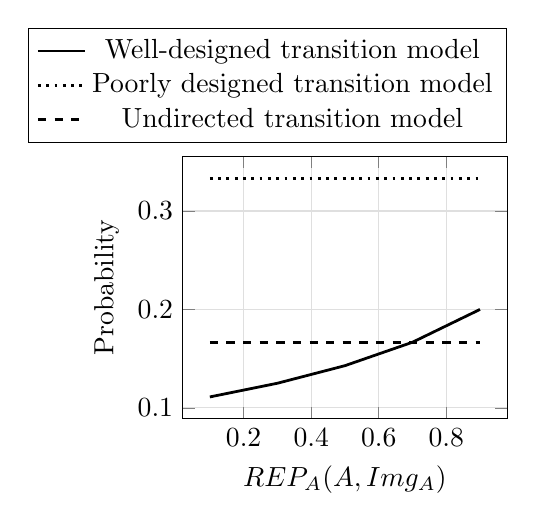
\begin{tikzpicture}
\begin{axis}[
    xlabel={$REP_A(A, Img_A)$},
	ylabel= Probability,
	title style={align=left},
	grid=both,
	minor grid style={gray!25},
	major grid style={gray!25},
	legend style={at={(1.0,1.05)},anchor=south east},
	width=0.47\linewidth,
	no marks
    ]
    
    
\addplot+[line width=1pt,solid,color=black] plot coordinates { (0.1, 1/9) (0.3, 1/8) (0.5, 1/7) (0.7, 1/6) (0.9, 1/5)};
\addlegendentry{Well-designed transition model};

\addplot+[line width=1pt,dotted,color=black] plot coordinates { (0.1, 1/3) (0.3, 1/3) (0.5, 1/3) (0.7, 1/3) (0.9, 1/3)};
\addlegendentry{Poorly designed transition model};

\addplot+[line width=1pt,dashed,color=black] plot coordinates { (0.1, 1/6) (0.3, 1/6) (0.5, 1/6) (0.7, 1/6) (0.9, 1/6)};
\addlegendentry{Undirected transition model}; 

\end{axis}
\end{tikzpicture}
}
\quad
\subfloat[Refusing trade offers]
{
\label{subfig:prof4}
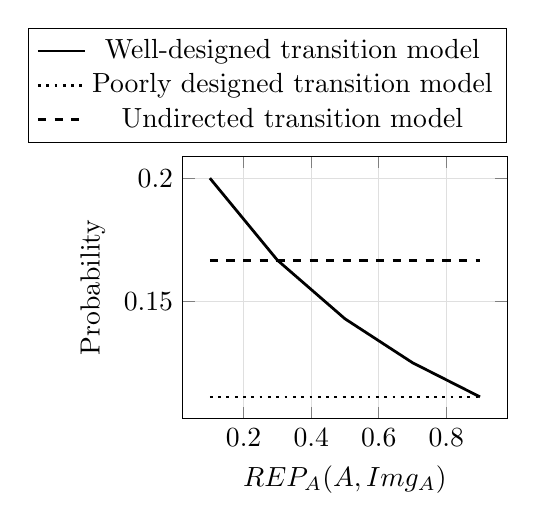
\begin{tikzpicture}
\begin{axis}[
    xlabel={$REP_A(A, Img_A)$},
	ylabel= Probability,
	title style={align=left},
	grid=both,
	minor grid style={gray!25},
	major grid style={gray!25},
	legend style={at={(1.0,1.05)},anchor=south east},
	width=0.47\linewidth,
	no marks
    ]
\addplot+[line width=1pt,solid,color=black] plot coordinates { (0.1, 1/5) (0.3, 1/6) (0.5, 1/7) (0.7, 1/8) (0.9, 1/9)};
\addlegendentry{Well-designed transition model};

\addplot+[line width=1pt,dotted,color=black] plot coordinates { (0.1, 1/9) (0.3, 1/9) (0.5, 1/9) (0.7, 1/9) (0.9, 1/9)};
\addlegendentry{Poorly designed transition model};

\addplot+[line width=1pt,dashed,color=black] plot coordinates { (0.1, 1/6) (0.3, 1/6) (0.5, 1/6) (0.7, 1/6) (0.9, 1/6)};
\addlegendentry{Undirected transition model};

\end{axis}
\end{tikzpicture}
}
\caption{Perceived probability of agent $B$ accepting and refusing the trade offers, as a function of the self-reputation of agent $A$.}
\end{figure}




\subsection{Adaptability of the RepNet framework}
\label{sub:adaptrep}


The second part of the experimental evaluation tests the ability of RepNet agents to adapt to changes in the behavior of other agents in the network when adaptation needs to happen quickly. In the previous set of experiments, while agent $B$ had a negative impact on agent $A$ when it refused each trade offer, $A$ could, in theory, turn around the situation, however bad it may be. Said differently, no state in the transition model represented a \textit{trap} that is impossible to escape. 
In \RefEx{ex:air1}, the scenario used in this section, if one agent starts monopolizing the vertiport for more time-steps than are necessary, the other agent is expected to quickly change its strategy in a way that minimizes the chances of crashes occurring. Failing to do so could result in the second agent not being able to land when absolutely necessary. From an implementational point of view, a crash is represented as a \textit{trap} state, and is, therefore, to be avoided at all costs.


To test the adaptability of RepNet agents, agent $A$ is managed by the RepNet algorithm, while agent $B$ is controlled by a simple algorithm that gradually increases the average time it spends on the vertiport. Agent $A$ is expected to be able to pick up on these changes and adapt its own behavior accordingly.
Specifically, agents $A$ and $B$ both start in the airspace, with their batteries fully charged. Agent $B$ is designed to initially only make use of the vertiport when absolutely necessary, i.e., when its battery is low. Every $10$ time-steps, Agent $B$'s selfishness is increased by a fixed factor $\xi \in [0,1]$. Concretely, $\xi$ represents the probability of agent $B$ deciding to stay at the vertiport for the following time-step. As the battery is fully recharged immediately upon landing at the vertiport, deciding to stay on the ground is perceived as a selfish and unnecessary move by agent $B$. 
2 series of 15 consecutive runs of 50 time-steps are conducted as follows:
\begin{itemize}
    \item The first series of runs aims at tracking the number of crashes that occur as a function of the number of time-steps. As the selfishness of agent $B$ increases, the likelihood of a crash does so as well.
    \item In the second series of experiments, agent $B$'s behavior is altered slightly: it will never choose to remain on the ground when agent $A$'s battery is low. This change makes it possible to uninterruptedly observe the behavioral changes of the RepNet agents across the 50 time-steps.
\end{itemize}
In an effort to provide an idea of how robust to changes in the behavior of agent $B$ the RepNet agent is, the same experiment is conducted under the same circumstances with agent $A$ now controlled by a standard \textit{MDP look-ahead} algorithm (\RefSec{sec:stateart}). Standard MDP-based algorithms are, by definition, incapable of adapting to behavioral changes of other agents, as these changes would have to be reflected in updates to the transition model. This MDP-based algorithm, therefore, serves as a baseline for comparison in this experiment.

As the \textit{immediate reward function} $\mathcal{R}$ of MDP agents is different from the \textit{perceived immediate impact} $PI$ of RepNet agents, the reward function was defined to be equal to the initial perceived impact of the RepNet agent, i.e.:
\begin{align}
    \forall s \in \mathcal{S}, \forall a \in \mathcal{A}: \mathcal{R}(s,a) = PI_g(s, AD_g^0, a)
\end{align}
where $AD_g^0(h,s)(a) = \frac{1}{|\mathcal{A}|} \,\, \forall h \in \mathcal{G}, \forall s \in \mathcal{S}, \forall a \in \mathcal{A}$. 



%The same experiment is furthermore conducted with the model-free learning algorithm called Q-Learning, using the $\epsilon$-greedy \textit{exploration-exploitation} strategy. The Q-Learning algorithm, although not designed to be used in dynamic environments, is, due to its ability to implicitly learn the transition through experience, expected to be robust \textit{to some degree} to gradual changes in the environment dynamics. \textcolor{red}{Not present yet}

The RepNet agent is expected to be able to sacrifice its selfish intentions, which would be to use the vertiport when in the air and leave the vertiport after landing, in an effort to avoid crashes.


\subsection{Large-scale experiments}
\label{sub:largeexp}
In the final part of the experimental evaluation, the ability of the RepNet algorithm to deal with an increased number of selfish agents is tested. To this end, Examples \ref{ex:trade3ag} and \ref{ex:air2} from the test bed are used hereafter. 

\subsubsection{Large-scale trading experiment}
\RefEx{ex:trade3ag} is used to verify the ability of a RepNet agent, say agent $A$, to manage its trades with the two remaining agents $B$ and $C$ (control agents), based not only on their behavior towards the agent of interest but also their behavior with each other. In fact, the action distribution, image, and reputation are general constructs, that is, they are not limited to tracking interactions that impact the RepNet agent \textit{directly}. 

The experiment can be divided into three parts: in the first part, agent $B$ is asked to refuse each trade offer made by agent $A$, while agent $C$ is expected to accept each trade offer coming from that same agent. This portion of the experiments assesses the ability of the RepNet agent (agent $A$) to accurately determine which agent it is more likely to successfully engage in trades with. In the second part, the roles are switched, and agent $B$ accepts the trade offers, while agent $C$ refuses them. This portion assesses the ability of the agent of interest to \textit{unlearn} what it has learned and adapt its behavior accordingly. 
In the third and final part, the RepNet agent's actions are \textit{blocked} from having any effect on the environment, preventing said agent from accumulating knowledge based on communications it is directly affected by. Furthermore, agents $B$ and $C$ are asked to engage in trades with each other. Agent $B$ is asked to reject all trade offers, while agent $C$ is asked to accept all trade offers. This portion of the experiment aims at testing the ability of the RepNet agent to draw conclusions on how it should act based on interactions it is not directly affected by. In fact, while the RepNet agent's actions have no effect on the environment, they are still recorded in this experiment and provide insight into which agent it is more likely to trade with. As the results described in \RefChap{chap:res} will show, Agent $A$ is, in fact, unable to adapt its behavior in these instances.


\subsubsection{Large-scale air-taxi experiment}
A final experiment is conducted using \RefEx{ex:air2} as the testing ground. The goal of this experiment is to demonstrate the ability of multiple RepNet agents to learn to cooperate with one another, despite their selfish intentions \cite{2590}. This experiment ties into the notion of \textit{convergence} in \textit{Multi-agent learning} (MAL), which was briefly discussed in \RefSec{sec:additional}. In particular, three of the four agents are controlled by their respective instances of the RepNet algorithm, while the last agent is controlled by a \textit{control} algorithm. Concretely, the control agent is initially tuned to be entirely selfless, i.e., it will always prioritize the other agents reaching their destination \textit{first} over reaching its own vertiport itself. Every $20$ time-steps, the selfishness of the fourth agent is gradually increased by a constant factor $\xi \in [0,1]$. $\xi$ represents the probability with which the control agent decides to move forward in situations in which the selfless move would be to stay in place. The RepNet agents are expected to notice these behavioral changes and adapt their own behavior accordingly. In doing so, they, however, alert the remaining RepNet agents of their own behavior change, forcing them to take these changes into account as well. 
The experiment itself runs for 100 time-steps. The agents are initially randomly dropped in the environment somewhere along their axis of travel. Each time every agent reaches its designated vertiport, the successful run is recorded, and the agents are randomly placed back in the environment. Each time a crash occurs, the unsuccessful run is recorded, and the agents are likewise randomly placed back in the environment. 


\label{sub:largescale}
\section{General parameters}
\label{sec:params}

\subsection{RepNet parameters}

\subsubsection{The image update function $\mathcal{U}$}
\label{sub:updatenn}

Given a current image value $v = Img_A(B,C)$ describing the image $C$ has of $B$, according to $A$, a learning rate $\alpha$, and the expected impact $i = ETI_A(B,C,s,AD_A)$ that $C$ has on $B$ when performing one of its actions in current the state $s$, $\mathcal{U}(\alpha, v, i)$ (\RefDef{def:systempo}) returns the updated value $v' = Img_A'(B,C)$. Agent $A$'s behavior is dictated by the image it believes each agent in the network to have of each other. Consequently, the image update function $\mathcal{U}$ has an important impact on $A$'s performance.
Two instantiations of the update function $\mathcal{U}$ are proposed by \textit{Rens et al.} \cite{rensetal}, namely the \textit{difference} update and the \textit{saturation} update.  

\begin{itemize}
    \item Difference update: 
    \begin{align}
    \mathcal{U}(\alpha, v, i) :=
        \begin{dcases}
            v + \alpha (1-v)i &\text{ if } i \geq 0
            \\
            v + \alpha (1+v)i &\text{ if } i < 0
        \end{dcases}
    \end{align}
    
    \item Saturation update: 
    \begin{align}
    \mathcal{U}(\alpha, v, i) :=
        \begin{dcases}
            1 &\text{ if } v + \alpha i > 1
            \\
            -1 &\text{ if } v + \alpha i < -1
            \\
            v + \alpha i &\text{ otherwise }
        \end{dcases}
    \end{align}
\end{itemize}

The update surfaces are shown in \RefFig{fig:upd} for $\alpha = 0.5$. The experiments discussed in this chapter were all conducted using the difference update, as it produced the most consistent results across all experiments. Note that this does not mean that the saturation update is of inferior quality. In fact, a small portion of the experiments was indeed found to work better with the saturation update, which is indicative of the domain-dependence of the \textit{image update function}. Nevertheless, in an attempt to keep the results consistent between tests, in particular those that make use of the same test bed, the same function was kept throughout the experimental evaluation.


\begin{figure}[h]
\subfloat[Difference update]
{
\label{subfig:update1}
    \includegraphics[width=0.48\textwidth]{images/MasterThesisUpdateDraw2.pdf}
}
\subfloat[Saturation update]
{
\label{subfig:update2}
    \includegraphics[width=0.48\textwidth]{images/MasterThesisUpdateDraw3.pdf}
}
\caption{Image update functions proposed by \textit{Rens et al.} \cite{rensetal}. The learning rate $\alpha$ is set to 0.5}
\label{fig:upd}
\end{figure}

\subsubsection{Expected total impact trade-off parameter $\delta$}
The trade-off parameter $\delta \in [0,1]$ in the expected total impact between agents $h$ and $i$ according to $g$, written $ETI(h,i,s,AD_g)$, trades off the relative importance of the impact due to agent $h$ and the impact perceived by $h$ (\RefDef{def:imp}). This parameter was set to $0.8$ across all experiments, that is, whenever $g$'s opinion on the image that $i$ has of $h$ ($Img_g(h,i)$) is updated, more weight will be given to the expected impact that $i$ has on $h$ in the current state, as opposed to the expected impact that $h$ has on $i$. Said differently, the image that a first agent $i$ has of another agent $h$ is conditioned mainly by $i$'s likeliness to impact (positively or negatively) $h$ in the current state $s$.

\subsubsection{Discount factor $\gamma$}
The discount factor $\gamma \in [0,1]$ in the RepNet framework's value function (\RefDef{def:opti}) determines the importance future time-steps should have on the agent's decision-making process. The closer it is to 1, the more important the future is, the closer it is to 0, the more important the present is. The value was set to 0.7 across all experiments.

\subsubsection{Initial settings for the action distribution and the image}
The RepNet agents deployed in a new environment are assumed to have no preconceived notions of other agents' behavior, reputation, and image of one another. This translates to the following initial settings for the action distribution and image for agent $g$:
\begin{align}
\begin{split}
    AD_g^0(h,s)(a) = \frac{1}{|\mathcal{A}|} \,\,\,\, \forall h \in \mathcal{G}, \forall s \in \mathcal{S}, &\forall a \in \mathcal{A},
    \\Img_g(h,i) = 0 \,\,\,\, \forall h, i \in \mathcal{G}, h \neq &i.
\end{split}
\end{align}

\subsection{MDP parameters}
\subsubsection{Discount factor $\gamma$}
The discount factor $\gamma \in [0,1]$ in the MDP framework's value function plays the same role as in the RepNet framework and was likewise set to 0.7 across all experiments involving an MDP agent.

\subsubsection{Look-ahead depth $D$}
The scenarios in which an MDP agent is used feature a look-ahead depth $D = 3$, as the same depth is used for the RepNet agents in said scenarios.


\section{Experiment-specific parameters}
\label{sec:specif}
Several parameters were tailored to each experiment separately. This section aims at summarizing the settings for these parameters. 

As such, $D$ is defined as the look-ahead depth of the online search algorithm used by RepNet agents (\RefSec{sec:onlineplan}). The higher it is, the more informed the RepNet agent's decisions can be. This comes at the drawback of increased computation times. \RefSec{sub:updatenn} reviewed the concept of image update function. This function takes a parameter $\alpha \in [0,1]$ called the learning rate that determines how quickly the image function is updated. $\eta$ is the \textit{Laplace} smoothing parameter and was introduced in \RefSec{sec:reduct} in an effort to smooth out the action distribution, especially in cases where the transition models are deterministic.

The only parameter that has not been discussed thus far is the \textit{exploration-exploitation trade-off parameter} $\epsilon$. In order for the RepNet agent to learn, sometimes it must be forced to try out actions even if the associated value is significantly lower than that of another action. In fact, in the trading examples between agents $A$ and $B$, if $A$ realizes $B$'s unwillingness to accept the trade offers, the value associated with the \texttt{trade\_with\_B} action decreases. If now $B$ changes its strategy and accepts all trade offers, $A$ can not know of this change unless it attempts to trade with $B$ occasionally. This concept is known in the literature as the \textit{exploration-exploitation trade-off} \cite{cassano2019isl}. \textit{Exploration} refers to the phase in which an agent performs actions that it would otherwise consider to be sub-optimal. \textit{Exploitation} refers to the phase in which an agent utilizes its current policy to move about in the environment. Several strategies for balancing \textit{exploration} and \textit{exploitation} exist, some simpler, others more complex. As the primary goal of this thesis does not lie in evaluating the benefits and drawbacks of different strategies, the arguably simplest strategy, called $\epsilon$-greedy, was used \cite{epsi}. The $\epsilon$-greedy strategy consists in selecting a random action $a \in \mathcal{A}$ at each time-step with a fixed probability $\epsilon \in [0,1]$, instead of selecting the action $a^\star$ that would, given the current policy, be considered optimal. The $\epsilon$-greedy strategy was solely utilized in the trading experiments, as using it with the air-taxi experiments can easily lead to crashes, and thus tarnish the significance of the results.
The settings for each parameter and experiment are summarized in Table \ref{tab:t1}.
\begin{table*}[h]
\centering
\begin{tabular}{c c c c c}
    \toprule
    \midrule
    \multirow{2}[4]{*}{Trading between 2 agents} & \multicolumn{4}{c}{Parameters}\\ 
    \cmidrule(rl){2-5}
    & $D$  & $\epsilon$ & $\alpha$ & $\eta$ \\ 
    \cmidrule(r){1-1}\cmidrule(l){2-5}
    \multicolumn{1}{l}{RepNet agent $A$}& 3 & 0.2 & 0.8 & 0.1   \\
    \midrule
    
    \multirow{2}[4]{*}{Trading between 3 agents} & \multicolumn{4}{c}{Parameters}\\ 
    \cmidrule(rl){2-5}
    & $D$  & $\epsilon$ & $\alpha$ & $\eta$  \\ 
    \cmidrule(r){1-1}\cmidrule(l){2-5}
    \multicolumn{1}{l}{RepNet agent $A$}& 3 & 0.2 & 0.8 & 0.1   \\
    \midrule
    
    \multirow{2}[4]{*}{Air-taxi with 2 agents} & \multicolumn{4}{c}{Parameters}\\ 
    \cmidrule(rl){2-5}
    & $D$  & $\epsilon$ & $\alpha$ & $\eta$  \\ 
    \cmidrule(r){1-1}\cmidrule(l){2-5}
    \multicolumn{1}{l}{RepNet agent $A$}& 3 & 0 & 1 & 0.15   \\
    \midrule
    
    \multirow{2}[4]{*}{Air-taxi with 4 agents} & \multicolumn{4}{c}{Parameters}\\ 
    \cmidrule(rl){2-5}
    & $D$  & $\epsilon$ & $\alpha$ & $\eta$   \\ 
    \cmidrule(r){1-1}\cmidrule(l){2-5}
    \multicolumn{1}{l}{RepNet agent $A$}& 2 & 0 & 1 & 0.1   \\
    \multicolumn{1}{l}{RepNet agent $B$}& 2 & 0 & 1 & 0.1   \\
    \multicolumn{1}{l}{RepNet agent $C$}& 2 & 0 & 1 & 0.1   \\
    \midrule
    \bottomrule
\end{tabular}
        %\centering
\caption{Settings for the experiment-specific parameters, for each of the experiments.}
\label{tab:t1}
\end{table*}
